\chapter{Literature Review}
The main purpose of this chapter is to present the needed theoretical and technical background to understand how the plugin works. Therefore, a short but sufficient definition of various concepts and tools will be given. In terms of theoretical context, this chapter will discuss topics like  Event-B, Maude and the rewriting logic approach to Event-B. Furthermore, this chapter will also provide some insight into plugin development in Rodin. To guide the reader through the different sections of this chapter and facilitate its reading, the following section dependency is given:

%insert image of section dependencies


\section{Event-B}

\section{Probabilistic Event-B}

\section{Maude}
%Main sources for this chapter: PeterMaude, Lecture1, Lecture3

%explain the generality of Maude
Maude is a high performance declarative language, that allows the specification of programs or systems, and their formal verification \cite{MaudeManual, Lecture1, PeterMaude}.
%explain how Maude program are written in functional module (sorts, subsorts, ops, etc, equations and equation evaluation)
Maude programs are represented as \textit{functional modules} declared with syntax:
\begin{lstlisting}
fmod MODULENAME is
    BODY
endfm
\end{lstlisting}
where \textit{MODULENAME} is the name of the functional module, and \textit{BODY} is a set of declarations that specify the program. The body of the module contains \textit{sorts} (written in Maude as \texttt{sorts}), where each sort correspond to an specific data type of the program. It also contains a set of function symbols or function declarations called \textit{operators} (abbreviated as \texttt{op} in Maude), that specify the constructors of the different sorts, along with the syntax of the program functions. Finally, a set of \textit{equations} (abbreviated as \texttt{eq} in Maude) is used to define the behavior of the functions. These equations use \textit{variables} (abbreviated as \texttt{var} in Maude) to describe how each function works. 

%provide an example of a maude program functional module
To illustrate how a Maude program is contructed, the following code corresponds to a program that defines the natural numbers and the addition operation, borrowed from \cite{PeterMaude}: 
\begin{lstlisting}
fmod NAT-ADD is
  sort Nat .

  op 0 : -> Nat [ctor] .
  op s : Nat -> Nat [ctor] .
  op _+_ : Nat Nat -> Nat .

  vars N M : Nat .
    
  *** Recursive Definition for addition
  eq N + 0 = N .
  eq N + s(M) = s(N + M) .
endfm
\end{lstlisting}
The sort \texttt{Nat} is a data type that represents the natural numbers. This sort has two constructors (represented in the code with the key word \texttt{ctor}): 0 which is a constant and the operator \texttt{s}, which takes one argument of type \texttt{Nat} and represents the successor function in the natural numbers. With these two operators, it is possible to define arithmetic functions in the natural numbers, like addition or multiplication. In this module, both functions are defined inductively using equations. Using this module, it is possible to compute the value for addition or multiplication for two natural numbers using the command \texttt{red}. For example, if the command \texttt{red s(s(s(0))) + s(s(0))} is used, that represents the operation 3 + 2, the answer 5 is obtained represented as \texttt{s(s(s(s(s(0)))))}:
\begin{lstlisting}
*********** equation
eq N + s(M) = s(N + M) .
N --> s(s(s(0)))
M --> s(0)
s(s(s(0))) + s(s(0))
--->
s(s(s(s(0))) + s(0))
*********** equation
eq N + s(M) = s(N + M) .
N --> s(s(s(0)))
M --> 0
s(s(s(0))) + s(0)
--->
s(s(s(s(0))) + 0)
*********** equation
eq N + 0 = N .
N --> s(s(s(0)))
s(s(s(0))) + 0
--->
s(s(s(0)))
result Nat: s(s(s(s(s(0)))))
\end{lstlisting}
Maude computes using equations from left to right. Therefore computation steps like the first one, the expression \texttt{s(s(s(0))) + s(s(0))} is matched with the left side of the equation \texttt{N + s(M) = s(N + M)} and matching substitution $\{\texttt{N} \mapsto \texttt{s(s(s(0)))},\texttt{M} \mapsto \texttt{s(0)} \}$. The resulting expression \texttt{s(s(s(0))) + s(s(0))}, will be simplified again with the same equation, until it reduces to a simplified expression that can be matched with the equation \texttt{N + 0 = N} (as seen in the last step).

%explain the semantics behind the functional modules
Semantically, functional modules in Maude are represented as \textit{equational theories} \cite{Lecture1,PeterMaude}, that are represented as a pair $(\Sigma, E)$ where: 
\begin{itemize}
    \item the \textit{signature} $\Sigma$ describes the syntax of the theory, which is the data types and operators symbols (sorts and operators).
    \item $E$ is the set of equations between expressions written in the syntax of $\Sigma$.
\end{itemize}
As mentioned before, computations in Maude are done by using the equations over expressions constructed with operators. This method is called \textit{term rewriting} \cite{Lecture1,PeterMaude} and behaves in the following way: 

\begin{itemize}
    \item With the equations $E$ of $(\Sigma, E)$, \textit{term rewriting rules} are defined as $\vv{E} = \{u \rightarrow v  \ | \ (u = v) \in E \}$. 
    \item A term $t$, which are expressions formed using the syntax in $\Sigma$, is rewritten to $t'$ in one step $t \rightarrow_{\vv{E}} t'$ if and only if, the following conditions are suffice:
        \begin{itemize}
            \item there is a subterm $w$ in $t$, expressed as $t[w]$.
            \item there is a rule $(u \rightarrow v) \in \vv{E}$ and a substituon $\theta$ s.t. : $w = u\theta$, $w' = v\theta$, $t'=t[w']=t[v\theta]$.   
        \end{itemize}
\end{itemize}
for example, in the previous computation \texttt{red s(s(s(0))) + s(s(0))} the term rewriting process in the second step, is the following:
\begin{itemize}
    \item $E = \texttt{N+s(M)=s(N + M)}$
    \item $t = \texttt{s(s(s(s(0))) + s(0))}$
    \item $\theta = \{\texttt{N} \mapsto \texttt{s(s(s(0)))},\texttt{M} \mapsto \texttt{0} \}$
    \item $w = \texttt{N+s(M)}\theta = \texttt{s(s(s(0))) + s(0)}$
    \item $w' = \texttt{s(N+M)}\theta = \texttt{s(s(s(s(0))) + 0)}$
    \item $t' = \texttt{s}([w']) = \texttt{s(s(s(s(s(0))) + 0))}$
\end{itemize}
the resulting term rewriting is $t \rightarrow_{\vv{E}} t'$.
%explain the functional modules with rewriting rules
%explain theory behind it
Aside from building programs in Maude using functional modules, it is also possible to model concurrent systems. This is done with \textit{system modules}, which permits the construction of system states and transitions. Semantically, a system module is a \textit{rewrite theory} \cite{PeterMaude,Lecture3} $\mathscr{R} = (\Sigma, E, L, R)$ where: 
\begin{itemize}
    \item $(\Sigma, E)$ is an equational theory.
    \item $L$ is a set of labels.
    \item $R$ is a set of unconditional labeled rewrite rules of the form $l: t \rightarrow t'$, and conditional labeled rewrite rules fo the form $l: t \rightarrow t' \ \text{if} \ cond$, where $l \in L$, $t,t'$ are terms in $\Sigma$ and $cond$ is a condition or system guard.    
\end{itemize}
The syntax for system modules in Maude is:
\begin{lstlisting}
mod MODULENAME is
    BODY
endm
\end{lstlisting}
Where the body represents a rewrite theory $\mathscr{R}$. The syntax for unconditional rewriting rules is
\begin{lstlisting}[mathescape=true]
rl [$l$] : $t$ => $t'$ .
\end{lstlisting}
and for conditional rewriting rules is
\begin{lstlisting}[mathescape=true]
crl [$l$] : $t$ => $t'$ if $cond$ .
\end{lstlisting}
%provide an example of a model
to exemplify this, lets consider the following simple model of a bus: A transport bus has capacity for 60 people. The bus can be moving or stationary and can only drop or lift passengers when the bus is stationary. Finally, at any time the bus driver can use the brake to stop or use the gas pedal to move. The corresponding Maude system module for this model is:
\begin{lstlisting}
mod BUS is protecting NAT .
  sorts Bus Status .

  op bus : Nat Status -> Bus [ctor] .
  ops stationary moving : -> Status [ctor] .
 
  vars N M : Nat . var S : Status .

  *** move the bus
  rl [move] : bus(N,stationary) => bus(N,moving) .
  *** stop the bus 
  rl [stop] : bus(N,moving) => bus(N,stationary) .
  *** drop passenger
  rl [drop] : bus(s(N),stationary) => bus(N,stationary) .
  *** lift passenger
  crl [lift] : bus(N,stationary) => bus(s(N),stationary) 
                                    if s(N) <= 60 . 
endm
\end{lstlisting}
%explain how the maude model corresponds to the theory
In this model the states of the system are represented with instances of the sort \texttt{Bus}, and it contains a natural number that represents the number of people inside the bus and a \texttt{Status}, which represents the state of the bus (it can be stationary or moving). In this case, no equations are used, therefore the set of equations $E = \emptyset$  and $\Sigma$ will contain the sorts \texttt{Bus} and \texttt{Status} with their respective operators. To model the different events in the model, 4 rewriting rules were used:
\begin{itemize}
    \item An unconditional rule labeled \texttt{move}, that represents the event of using the gas pedal to move the bus by changing the status from \texttt{stationary} to \texttt{moving}. Note that this rule can only be applied when the bus is \texttt{stationary}, as stated by the rule first term \texttt{bus(N,stationary)}.
    \item An unconditional rule labeled \texttt{stop}, that represents the event of using the brakes to stop the bus. This changes the status of the bus from \texttt{moving} to \texttt{stationary}. As the previous rule, it can only be applied when the first term is matched, i.e. when the bus status is \texttt{moving}. 
    \item An unconditional rule labeled \texttt{drop}, that represents the event of dropping people off the bus. The subterm \texttt{s(N)} assures that the it can only drop a person when the number of people in one or more. This rule rewrites the state of the system, by reducing the number of passengers in the bus by one.
    \item A conditional rule labeled \texttt{lift}, that represents the event of lifting a passenger. When this rules is applied, the number of passengers inside the bus is increased by one. To prevent exceeding the maximum capacity of the bus, the condition \texttt{if s(N) <= 60} is used. 
\end{itemize}
With this system module, that represents a rewrite theory $\mathscr{R}$, the simple bus model can be specified and verified using other functionalities in Maude like model checking with the commands \texttt{rew} and \texttt{search} \cite{MaudeManual}.


\section{Object-Based Programming in Maude}



\section{PMaude}
%acknowledge the PMaude paper
%explain what PMaude is (probably use the thesis proposal)
Probabilistic Maude or PMaude \cite{Agha2006}, is a Maude extension that introduces probabilities to the language. The underlying theory behind PMaude are  \textit{probabilistic rewrite theories} which correspond to an extension of rewrite theories: probabilistic rewrite theories can be expressed as tuple $\mathscr{R}_p = (\Sigma, E, L, R, \pi)$, where $(\Sigma, E, L, R,)$ is a rewrite theory and $\pi$ is a function that assigns to each rewrite rule $r \in R$ a probability, given the current model state or configuration. This probability will determine if a rule may or may not be executed in the following system transition. The general form of probabilistic rewrite rules, for unconditional and conditional respectively is:
\begin{align*}
    l &: t(\overrightarrow{x}) \rightarrow t'(\overrightarrow{x}, \overrightarrow{y}) \; \text{if} \; C(\overrightarrow{x}) \; \textbf{with probability} \; \overrightarrow{y} := \pi_r(\overrightarrow{y}) \\
    l' &: t(\overrightarrow{x}) \rightarrow t'(\overrightarrow{x}, \overrightarrow{y}) \; \textbf{with probability} \; \overrightarrow{y} := \pi_r(\overrightarrow{y})  
\end{align*}
Where $\overrightarrow{x}$ is the set of variables of the current model state,  $\overrightarrow{y}$ is the set of new variables accessible in the following model state and $C(\overrightarrow{x})$ is the conjunction of conditions over the set $\overrightarrow{x}$. Moreover, $l, l'$ are labels in $L$, $t,t'$ are terms written with $\Sigma$ and $\pi_r$ corresponds to the probability function assigned to the specific rule $r \in R$. 
%provide the clock example and explain it
Lets consider the PMaude module, presented in \cite{Agha2006}: 
\begin{lstlisting}[mathescape=true]
pmod EXPONENTIAL-CLOCK is
  *** the following imports positive real number module
  protecting POSREAL .

  *** the following imports PMaude module that defines 
  *** the distributions EXPONENTIAL, BERNOULLI, GAMMA, etc.
  protecting PMAUDE .

  *** declare a sort Clock
  sort Clock .
  *** declare a constructor operator for Clock
  op clock : PosReal PosReal => Clock .
  *** declares a constructor operator for a broken clock
  op broken : PosReal PosReal => Clock .

  *** T is used to represent time of clock,
  *** C represents charge in the clocks battery,
  *** t represents time increment of the clock
  vars T C t : PosReal . var B : Bool .
  
  rl [advance]: clock(T,C) =>
                      if B then
                           clock(T+t,C - $\frac{\text{C}}{1000}$)
                      else
                           broken(T,C - $\frac{\text{C}}{1000}$)
                      fi
                with probability B:=BERNOULLI($\frac{\text{C}}{1000}$) 
                                and 
                                t:=EXPONENTIAL(1.0).
                
  rl [reset]: clock(T,C) => clock(0.0,C) .
endpm
\end{lstlisting}
This model represents a clock that works with a battery. The idea is to model the behavior of the clock, when the battery starts depleting: when the charge of the battery is high, then the probability that the clock breaks is low. Conversely, when the clock's battery is low, the clock has a higher probability of breaking. In this probabilistic system module, the clock is represented as a term \texttt{clock(T,C)}, where \texttt{T} is the time and \texttt{C} is the charge of the clock. The main probabilistic rewrite rule \texttt{advance} represents the "ticks" of the clock. If the boolean value \texttt{B} is true, then the clocks ticks normally and the new time will be the current time \texttt{T} plus an increment \texttt{t}. Also, the charge of the clock will be reduced by a thousandth of the currents clock's charge. If \texttt{B} is false, then the clock will break and change to the state \texttt{broken(T,C - $\frac{\texttt{C}}{1000}$)}. The constructor \texttt{broken} of sort \texttt{Clock}, represents the broken state of the clock. To incorporate the probabilistic choice of event for the clock's state (either ticking or breaking), the value \texttt{B} is chosen probabilistically, based on the charge of the clock. This is done by the \texttt{BERNOULLI} function, which receives a float number and returns a boolean value that is distributed according to the Bernoulli distribution with mean $\frac{\texttt{C}}{1000}$. Therefore, the lesser the charge left in the battery, the greater is the probability that the clock will break. The value \texttt{t} is also probabilistically determined, in this case by a exponential distribution function.
There is also a second rewriting rule, that resets the clock to its initial state \texttt{clock(0.0, C)}. It is important to remark that this model has both probabilistic and non-deterministic choice: The state of the clock depends on a probability function but the choice of rewriting rules is done non-dereministically by Maude's fair scheduler.

PMaude modules can be transformed into regular system modules in Maude. This is done with three key modules: \texttt{COUNTER}, \texttt{RANDOM} and \texttt{SAMPLER}. The built-in \texttt{COUNTER} module in Maude consists of the rewriting rule
\begin{lstlisting}
rl counter => N:Nat .
\end{lstlisting}
that rewrites the constant counter to a natural number. The module is built to guarantee that every time the constant counter is replaced with a natural number \texttt{N}, this natural number corresponds to the successor of the natural number obtained in the previous use of the rule. The built-in \texttt{RANDOM} module provides a random number generator function, called \texttt{random}. Lastly, the \texttt{SAMPLER} module specifies the sampling functions for different probability functions. For example, for the previous clock example, the needed functions will be:
\begin{lstlisting}
op EXPONENTIAL : PosReal => PosReal .
op BERNOULLI : PosReal => Bool .
\end{lstlisting}
that are defined as:
\begin{lstlisting}
rl EXPONENTIAL(R) => (- log(rand)) / R .
rl BERNOULLI(R) => if rand < R then true else false fi .
\end{lstlisting}
The value \texttt{rand} in both of the rules is defined as:
\begin{lstlisting}
rl [rnd] : rand => float(random(counter + 1) / 4294967296) .
\end{lstlisting}
and it is rewritten in each step to a random number between 0 and 1. The number 4294967296 is used to divide the number returned by \texttt{random}, since it is the maximum number the function can return. The resulting Maude system module \cite{Agha2006} is:
\begin{lstlisting}[mathescape=true]
mod EXPONENTIAL-CLOCK-TRANSFORMED is 
  *** The SAMPLER mode includes the COUNTER and RANDOM modules
  protecting SAMPLER .
  protecting POSREAL .
  
  sort Clock . 
  op clock : Nat Float -> Clock [ctor] . 
  op broken : Nat Float -> Clock [ctor] . 
  
  vars T C : PosReal . 
  
  rl clock(T,C) => if BERNOULLI($\frac{\text{C}}{1000}$) then 
                        clock(T + EXPONENTIAL(1.0), C - $\frac{\text{C}}{1000}$) 
                   else 
                        broken(T,C - $\frac{\text{C}}{1000}$)
                   fi .
  
  rl [reset]: clock(T,C) => clock(0.0,C) .
endm
\end{lstlisting}

\section{PVeStA}
%explain what is pvesta
PVeStA \cite{AlTurki2011} is a statistical model checking tool for probabilistic-real time systems, that are specified either as discrete or continuous Markov chains, or probabilistic rewrite theories in Maude. It permits the verification of properties expressed in quantitative temporal logics like QuaTex \cite{Agha2006} using Monte Carlo simulations.
%exlpain how to it works (version of Maude, files, process to verify a PMaude model)
PVeStA is implemented in Java and consists of two executable programs: a client \texttt{pvesta-client} and a server \texttt{pvesta-server}. The \texttt{pvesta-client} program takes as input the Maude probabilistic model, a list of formulas written in QuaTex, multiple execution parameters for the model checking simulation and a server list. Then it sends to every one of the running \texttt{pvesta-servers} (PVeStA's model checking supports parallelism) a simulation request for the specified probabilistic Maue model and QuaTex formulas. After that, the servers return the results back to the \texttt{pvesta-client} program. This previously explained process can be viewed in the following figure:
\begin{figure}[h]
    \centering
    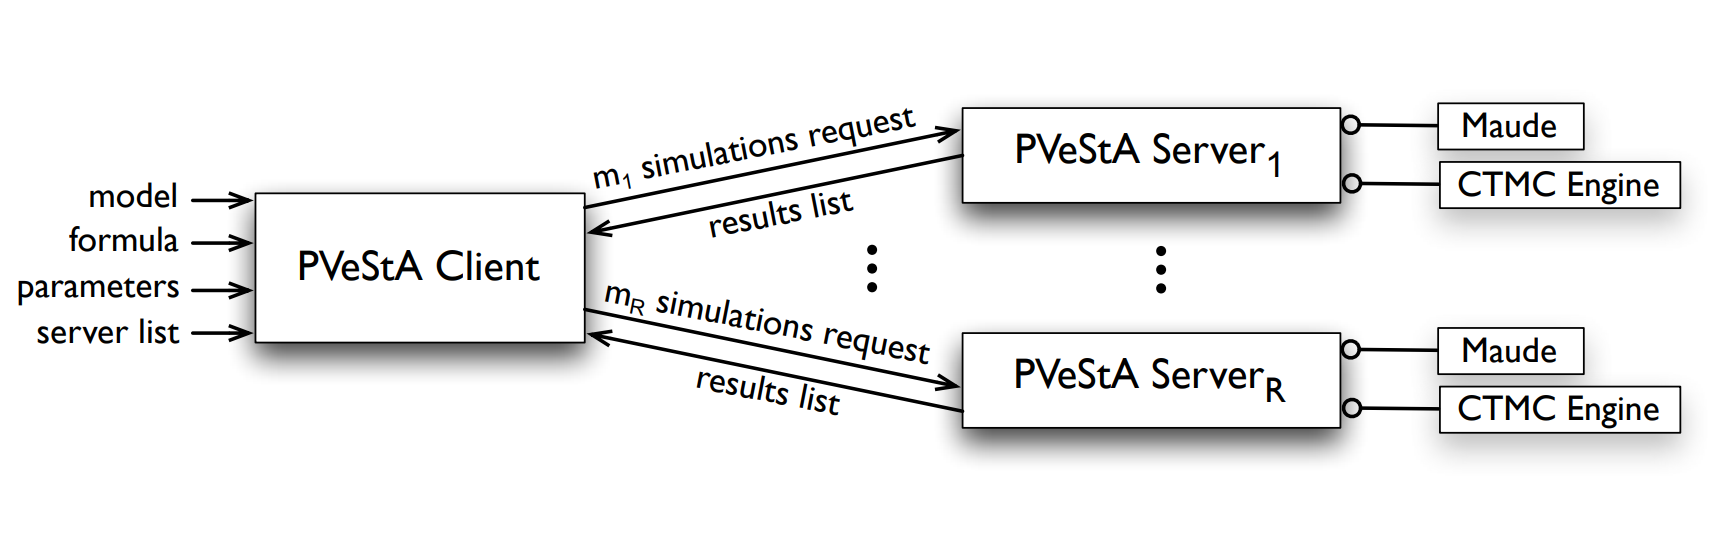
\includegraphics[scale = 0.3]{images/pvesta.PNG}
    \caption{Components and interactions of PVeStA, taken from \cite{AlTurki2011}}
    \label{fig:pvesta}
\end{figure}
To demonstrate how PVeStA works, a variation of the clock model shown in the previous section will be used. 






\section{A Rewriting Logic Semantics and Statistical Analysis for Probabilistic Event-B}

\section{Rodin and Plugin Development}










